%%%%%%%%%%%%%%%%%%%%%%%%%%%%%%%%%%%%%%%%%%%%%%%%%%%%%%%%%%%%%%%%%%%%%%%%%%%%%%%
% Titel:   Analyse
% Autor:   
% Datum:   13.12.2013
% Version: 0.0.1
%%%%%%%%%%%%%%%%%%%%%%%%%%%%%%%%%%%%%%%%%%%%%%%%%%%%%%%%%%%%%%%%%%%%%%%%%%%%%%%
%
%:::Change-Log:::
% Versionierung erfolgt auf folgende Gegebenheiten: -1. Release Versionen
%                                                   -2. Neue Kapitel
%                                                   -3. Fehlerkorrekturen
%
% 0.0.0       Erstellung der Datei
%%%%%%%%%%%%%%%%%%%%%%%%%%%%%%%%%%%%%%%%%%%%%%%%%%%%%%%%%%%%%%%%%%%%%%%%%%%%%%%    
\chapter{Analyse}\label{ch:analyse}
	Im folgenden Abschnitt werden die in Abschnitt \ref{ss:speilaufgaben} \textit{Spielaufgaben} beschriebenen Aufgaben analysiert und Strategievarianten entworfen und bewertet. Weiter werden einzelnen Bereiche des kleinen Roboters festgelegt, was f�r die Kommunikation und den restlichen Teilteams als Ausgangslage dient.
	%
	%
	% Strategie
	\section{Strategie}\label{s:strategie}
		Die Strategie wird �ber Erfolg und Misserfolg des gesamten Projektes entscheiden und muss dementsprechend behandelt werden.
		%
		\subsection{Ausgangslage}
			Das Eurobot 2014 Reglement stellt dieses Jahr 5 Aufgaben. Mit unseren Ressourcen ist es nicht m�glich alle Aufgaben zufriedenstellend  zu l�sen. Das Team hat sich zum Ziel gesetzt den Schweizermeistertitel nach Burgdorf zu holen. Aus den Ranglisten der letzten Jahre geht hervor, dass mit 30\% aller machbaren Punkte eine Platzierung unter den ersten drei erreicht werden m�sste. Diese 30\% Marke wird somit angestrebt. Es werden also zu erst die Aufgaben bestimmt, welche gel�st werden sollen. 	
		%
		\subsection{Vorgehen}
			Um die einzelnen Aufgaben zu analysieren und gleichzeitig die Kompatibilit�t mit anderen Aufgaben bewerten zu k�nnen wurde ein Formular erstellt. Das Bewertungstool ist auf dem Prinzip einer Risikoanalyse aufgebaut. Es soll aufzeigen welche Systeme realisierbar sind und wie viele Punkte erreicht werden k�nnen. Die Analyse beinhaltet folgende Kriterien (siehe Tabelle \ref{tab:bewertungskriterien}).
			%
			\begin{table}[htbp]
          		\centering
          		\begin{tabularx}{\textwidth}{|X|X|} 
					\hline
					\rowcolor{bfhblue}
					\textcolor{white}{Kriterien} & \textcolor{white}{Bemerkung}\\
					\hline
					Angestrebte Punkte mit und ohne Bonus & Absch�tzung der machbaren Punkte\\
					\hline
					Zeitaufwand (Handling) & Absch�tzung der Zeit die ben�tigt wird um die Aufgaben zu l�sen.\\
					\hline
					Fahrwege (Zeit / Hindernisse) & Absch�tzung der Zeit um die n�tigen Positionen anzufahren.\\
					\hline
					Risiko durch Gegner & Einsch�tzung der Wahrscheinlichkeit, dass der Gegner die Punkte verhindert.\\
					\hline
					Flexibilit�t (Intelligente Strategie) & L�sst das System die Integration von Taktischen Entscheidungen w�hrend des Spieles zu.\\
					\hline
					Entwicklungsaufwand Mechanisch / Elektronisch & Absch�tzung des Zeitaufwandes zur Realisierung\\
					\hline
					Fehleranf�lligkeit & Absch�tzung des Zeitaufwandes zur Realisierung\\
					\hline
				\end{tabularx}
          		\caption{Bewertungskriterien}
          		\label{tab:bewertungskriterien}  
      		\end{table}	
      		%
      		Damit eine Bewertung der jeweiligen Strategien m�glich wird sind zwei numerische Faktoren eingebaut worden:
      		%
      		\begin{description}
      			\item[Spezifische Punkte] Anzahl erwartete Punkte pro Zeiteinheit.
      			\item[Spezifischer Aufwand] Anzahl der total erwarteten Entwicklungsstunden pro Punkt.
      		\end{description}
      		%
      		Die eigentliche Bewertung und anschliessende Auswahl erfolgt in einer Nutzwertanalyse. Die Chancenanalysen sowie die Nutzwertanalyse sind im Anhang B \textit{Strategie} zu finden.	
      	%
      	\subsection{Resultat}
      		Der Entscheid f�llt schliesslich auf die Variante 1. Diese beinhaltet folgende Schwerpunkte:
      		%
      		\begin{itemize}
	      		\item 2-Roboter-Strategie
	      		\item Bau des prim�r Roboters in der \gls{ac:pa1}
	      		\begin{itemize}[parsep=1pt]
		      		\item Nach M�glichkeiten als kleiner Roboter bauen
		      		\item Hauptaufgaben:
		      		\begin{itemize}[parsep=1pt]
			      		\item Mammut jagen
			      		\item Fresko (Wandmalerei)
		      		\end{itemize}
	      		\end{itemize}
	      		\item Bau des sekund�r Roboters in der \gls{ac:pa2}
	      		\begin{itemize}[parsep=1pt]
		      		\item Baugr�sse je nach Entwicklungsgrad w�hlen. Option von zwei identischen Grundplatten bleibt offen.
		      		\item Hauptaufgaben:
		      		\begin{itemize}[parsep=1pt]
			      		\item Feuer sammeln
			      		\item Mammut fangen (Funny-Action)
		      		\end{itemize}
	      		\end{itemize}
      		\end{itemize}
      		%
      		Die beschriebene Strategie zeichnet sich insbesondere durch ein optimales Verh�ltnis zwischen Entwicklungsaufwand und erreichbaren Punkten aus. Da sie keine sehr komplizierten Handling Aufgaben l�st, ist auch die Fehleranf�lligkeit eher gering.\par 
      		%
      		F�r die Feueraufgabe wird nur wenig Entwicklungsaufwand vorgesehen. Im besten Fall kann diese aber bis zur Perfektion weiterentwickelt werden, da fast der komplette grosse Roboter zur Verf�gung steht.\par 
      		%
      		Die Alternative bestand aus einer Variante die den Schwerpunkt auf die Feueraufgabe legt. Hierbei sollte mittels einer Kamera und einer ausgefeilten Bildverarbeitung gearbeitet werden. Da die Bildverarbeitung aber als sehr Komplex eingestuft wird und somit das Risiko des Scheiterns bedeuten gr�sser wird, f�llt der Entscheid gegen diese Variante.
%	
%		\todo{Nullpunkt, Achsendefinition}
%		\image{content/image/3_spielfeldnavigation}{scale=1}[Spielfeld][abb:spielfeld]
%	\section{Spielmanipulation}{Hannes/Patrick}
    %
    %
    %Kleiner Roboter
    \section{Module Roboter}\label{s:module_roboter}
    	Der Roboter besteht aus verschiedenen Teilsystemen, die im Roboter zu einem gesamten System vereint werden. In Abbildung \ref{abb:gliederung_kleiner_roboter} auf Seite \pageref{abb:gliederung_kleiner_roboter} sind die verschiedenen Module des kleinen Roboters schematisch dargestellt.
    	%
    	%\image{content/image/3_module_im_roboter}{scale=0.7}[Gliederung kleiner Roboter][abb:gliederung_kleiner_roboter]
    	%
    	\begin{figure}[t]%H htbp
    		\centering
    		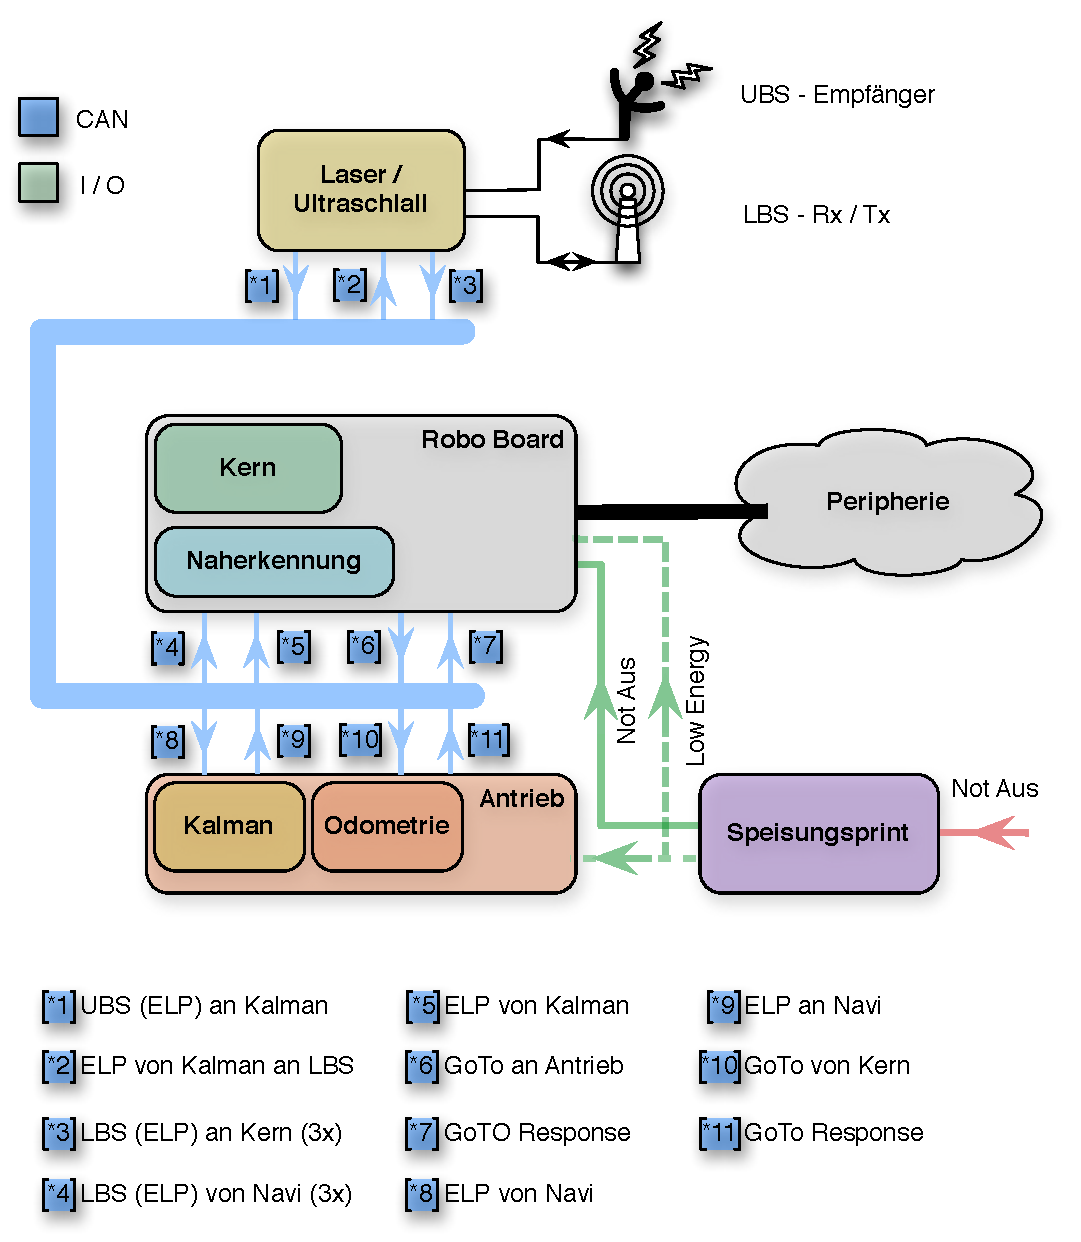
\includegraphics[scale=0.6]{content/image/3_module_im_roboter}
    		\caption{Gliederung kleiner Roboter}
    		\label{abb:gliederung_kleiner_roboter}
    	\end{figure}	
    	
		\begin{description}
			\item[Kernknoten] Der Kernknoten bestehend aus einem RoboBoard ist f�r die gesamte Steuerung des Roboters verantwortlich. Der Kernknoten �bernimmt die strategischen Abl�ufe, so wie die Kommunikation mit den anderen Modulen. Zus�tzlich ist im kleinen Roboter aus Platzgr�nden auch die Naherkennung auf dem Kernknoten umgesetzt.
			%
			\item[Navigation] Damit der Roboter zu jederzeit wissen kann, wo er sich befindet, muss eine Navigationseinheit umgesetzt werden. Diese wird mittels Ultraschall 		und / oder Laser umgesetzt. Wichtig beim Navigationsmodul ist, dass diese auch f�r die Kommunikation zwischen den Robotern verantwortlich sind.
			%
			\item[Antrieb] Der Antrieb ist eines der wichtigsten Module in unserem Roboter. Der antrieb steuert die Motoren an, rechnet Routen aus, um Zielpositionen zu erreichen und liest die Odometrie des Roboters aus. Weiter wird auf der Antriebseinheit das Kalmanfilter implementiert, welches die Positionsbestimmung des Roboters verbessern soll.
			%
			\item[Speisung] Da der Roboter mit 22.2 V Lithium Akkus gespiesen wird, ist es n�tig einen zus�tzlichen Speisungsprint zu verbauen, so dass auch  Spannungen wie 5 V Logik zur Verf�gung stehen. Der Speisungsprint �berwacht weiter die Akkuspannungen und kann im falle eines Not Aus die Stromzufuhr zu den Aktoren des Roboters kappen.
			%
			\item[Peripherie] Damit der Roboter mit der Umwelt interagieren kann, m�ssen verschiedene Sensoren und Aktoren angesteuert werden. Diese beschr�nken sich beim kleinen Roboter auf ein paar Servos, Taster und Sensoren f�r die Naherkennung.\par
		\end{description}
		%
		Damit die verschiedenen Module des Roboters miteinander Kommunizieren k�nnen, werden diese mittels CAN-Schnittstelle miteinander verbunden. Auf die Kommunikation wird im Abschnitt \ref{s:kommunikation} auf Seite \pageref{s:kommunikation} genauer eingegangen.